\chapter{Wissenschaftliche Grundlagen}
Für die Erarbeitung der Anwendung ist Vorwissen über graphische Strukturen nötig.
Die folgenden Abschnitte dienen der Erarbeitung dieses Vorwissens, sowie der Erklärung von verwendeten Programmen.

\section{Planare Graphen}
Der Grundriss wird mithilfe eines planaren Graphen beschrieben.               
Ein planarer, auch plättbarer Graph, ist ein Graph, der in einer Ebene mithilfe von Knoten und Kanten dargestellt werden kann, ohne dass sich zwei oder mehr Kanten schneiden (vgl. Quelle \cite{planarGraph}, siehe Abb.~\thebildnrnext). 
Jede Fläche des Graphen wird durch mindestens drei verschiedene Kanten beschrieben, die den Rand der Fläche markieren. 
Die Fläche um den Graphen herum, welche unbegrenzt groß ist, wird äußeres Gebiet genannt. \\

\begin{Bild}{Schema eines planaren Graphen (Abbildung der Verfasser)}
	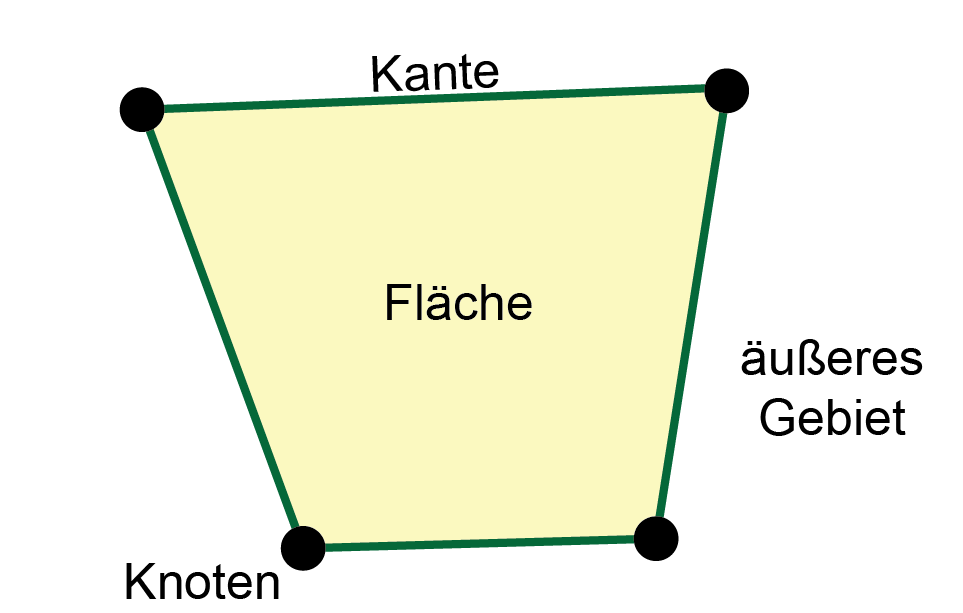
\includegraphics[width = 250px]{Bilder/planarerGraph-11}
\end{Bild}

\section{Doubly Connected Edge List}
Um planare Graphen ohne Informationsverlust zu speichern wird in der Informatik eine \q{Doubly Connected Edge List} (DCEL) genutzt.
In einer DCEL wird jeder Kante, die aus einem Anfangsknoten und Endknoten besteht, jeweils eine Vorgänger-, Nachfolger-, Zwillingskante und die angrenzende Fläche zugewiesen. 
Durch die Darstellung einer Linie des Grundrisses durch zwei zueinander entgegengesetzt laufenden Kanten wird gewährt, dass keine zwei Flächen an einer Kante anliegen.
Zudem wird für einen Knoten der DCEL eine ausgehende Kante und für eine Fläche eine anliegende Kante gespeichert (vgl. Quelle \cite{dcel} und \cite{dcelwiki}). \\
Die Kanten der Flächen verlaufen im mathematisch positiven Drehsinn.
Als einzige Ausnahme gilt das äußere Gebiet, welches einen mathematisch negativen Drehsinn besitzt. \\
In Abb.~\thebildnrnext\ ist eine solche DCEL zu sehen.
Die nachfolgenden Tabellen verdeutlichen die Referenzen der Bestandteilen der DCEL in Abb.~\thebildnrnext.\\

\begin{Bild}{Schema einer DCEL (Abbildung der Verfasser)}
	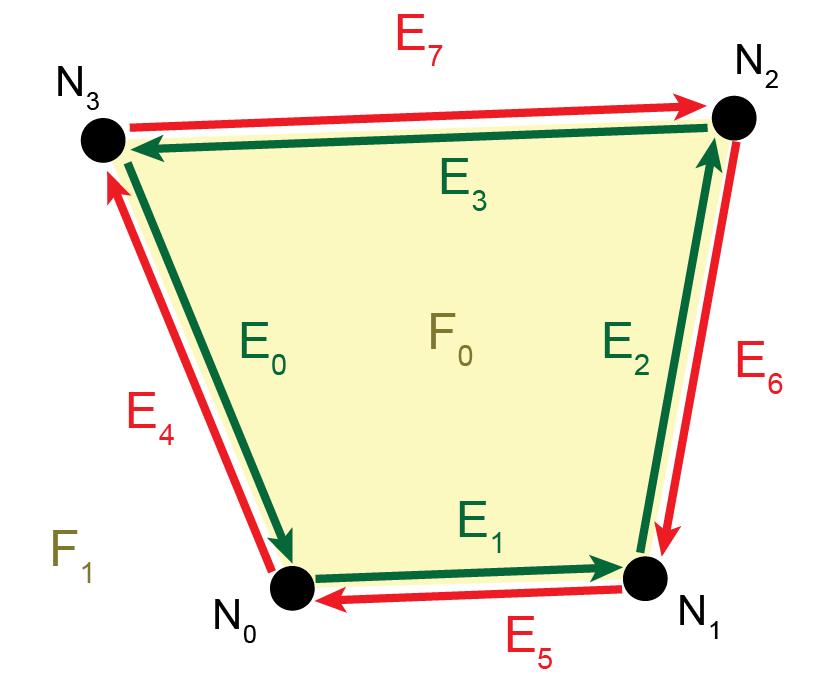
\includegraphics[width=250px]{Bilder/DCEL-10}
\end{Bild}

\begin{tabularx}{\textwidth}{|Y|Y|}
	\hline
	\thead{Knoten} & \thead{ausgehende Kante} \\
	\hline
	$N_0$ & $E_1$ \\
	\hline
	$N_2$ & $E_6$ \\
	\hline
\end{tabularx}\\\vspace{12px}

\begin{tabularx}{\textwidth}{|Y|Y|}
	\hline
	\thead{Fläche} & \thead{anliegende Kante} \\
	\hline
	$F_0$ & $E_3$ \\
	\hline
	$F_1$ (äußeres Gebiet) & $E_7$ \\
	\hline
\end{tabularx}\\

\begin{tabularx}{\textwidth}{|Y|Y|Y|Y|Y|}
	\hline
	\thead{Kante} & \thead{Nachfolger} & \thead{Vorgänger} & \thead{Zwilling} & \thead{Fläche} \\
	\hline
	$E_0$ & $E_1$ & $E_3$& $E_4$& $F_0$ \\
	\hline
	$E_1$ & $E_2$ & $E_0$& $E_5$& $F_0$ \\
	\hline
\end{tabularx}

\section{Oriented Minimum Bounding Box}
Die Oriented Minimum Bounding Box (OMBB) bzw. das orientierte minimale Begrenzungsrechteck einer Fläche ist das Rechteck, welches das komplette Polygon umschließt und dabei den kleinstmöglichen Flächeninhalt besitzt (siehe Abb.~\thebildnrnext).
Sie wird über den \q{Convex Hull} (konvexe Hülle) eines Polygons berechnet.
Die \q{Convex Hull} ist die kleinste konvexe Menge, in der die Punkte der Fläche enthalten sind (siehe Abb.~\thebildnrnext).
Mindestens eine Seite des minimalen Begrenzungsrechtecks ist kollinear zu einer Seite der konvexen Hülle (vgl. Quelle \cite{ombb}).

\begin{Bild}{Beispiel einer konvexen Hülle (vgl. Quelle \cite{ombb})}
	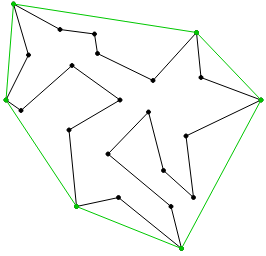
\includegraphics[width = 140px]{Bilder/convex_hull}
\end{Bild}
\begin{Bild}{Eine mögliche Bounding Box (l.) im Vergleich zur OMBB (r.) (vgl. Quelle \cite{ombb})}
	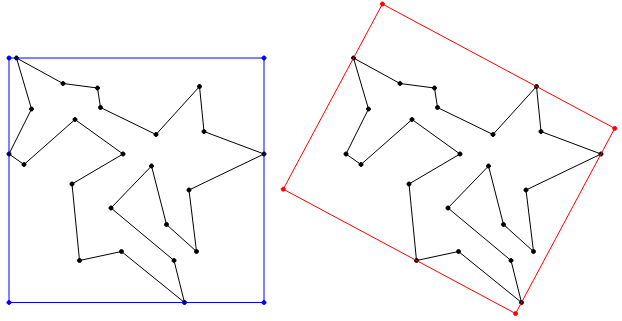
\includegraphics[width = 282px]{Bilder/aabb_vs_ombb}
\end{Bild}

\section{AutoCAD}
%Konstruktionsprogramm statt architektenprogramm
AutoCAD ist ein grafischer Zeichnungseditor, welcher zum Erstellen von technischen Zeichnungen und dem Modellieren von Objekten verwendet wird (vgl. Quelle \cite{autocadwiki}).
AutoCAD verwendet dabei einfache Objekte wie Linien, Kreise und Bögen, um auf deren Grundlage kompliziertere Objekte zu bilden.
Zu AutoCAD gehörig wurde das Dateiformat \q{.dxf} entwickelt, welches als Industriestandard zum Austausch von CAD-Dateien dient. \\

\begin{Bild}{Grundriss aus AutoCAD (Screenshot der Verfasser)}
	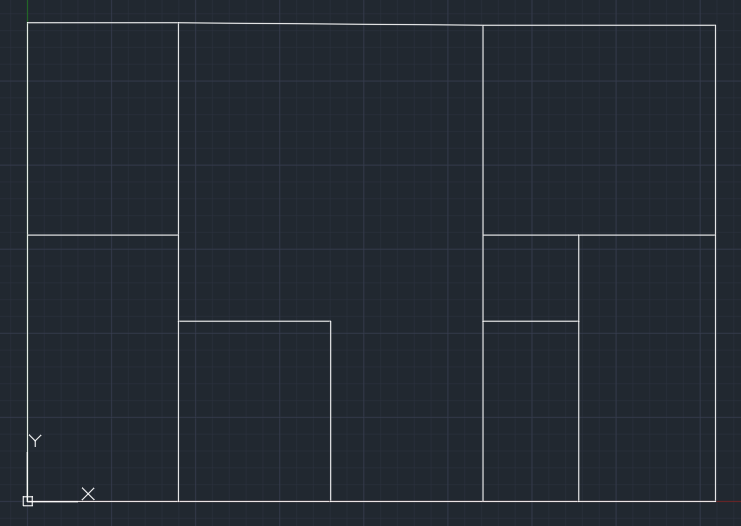
\includegraphics[width=300px]{Bilder/Grundriss}
\end{Bild}

Der Grundriss, der später als Ausgangspunkt fungiert, wird in AutoCAD erstellt und liegt als .dxf-Datei vor.
Ein Beispiel für einen solchen Grundriss ist in Abb.~\thebildnr\ zu sehen.

\section{OpenSCAD}
OpenSCAD ist eine kostenlos verfügbare CAD-Modellierungssoftware, welche aus einer textbasierten Beschreibungssprache 3D-Modelle erzeugt (vgl. Quelle \cite{OpenScad}).
OpenSCAD bietet dabei verschiedene Vorteile während des Modellierungsvorganges, beispielsweise das farbige Hervorheben oder die Modularisierung zusammenhängender Objekte. \\
%Modellierung
Die Modellierung von einfachen Basisobjekten in OpenSCAD erfolgt durch das Verwenden von Anweisungen wie \icode{cube()}, \icode{sphere()} oder \icode{cylinder()} und Parametern in Klammern.
Diese Basisobjekte können anschließend durch Mengenoperationen wie Vereinigungen (\icode{union()}), Differenzen (\icode{difference()}) oder Schnittmengen (\icode{intersection()}) und Transformationen wie Skalierungen (\icode{scale()}), Rotationen (\icode{rotate()}) oder Translationen (\icode{translate()}) miteinander verknüpft und kombiniert werden, um neue Objekte nach eigenen Ansprüchen zu erzeugen (siehe Abb.~\thebildnrnext). \\

\begin{Bild}{Differenzmenge zwischen einem Würfel und einem Zylinder in OpenSCAD (Screenshot der Verfasser)}
	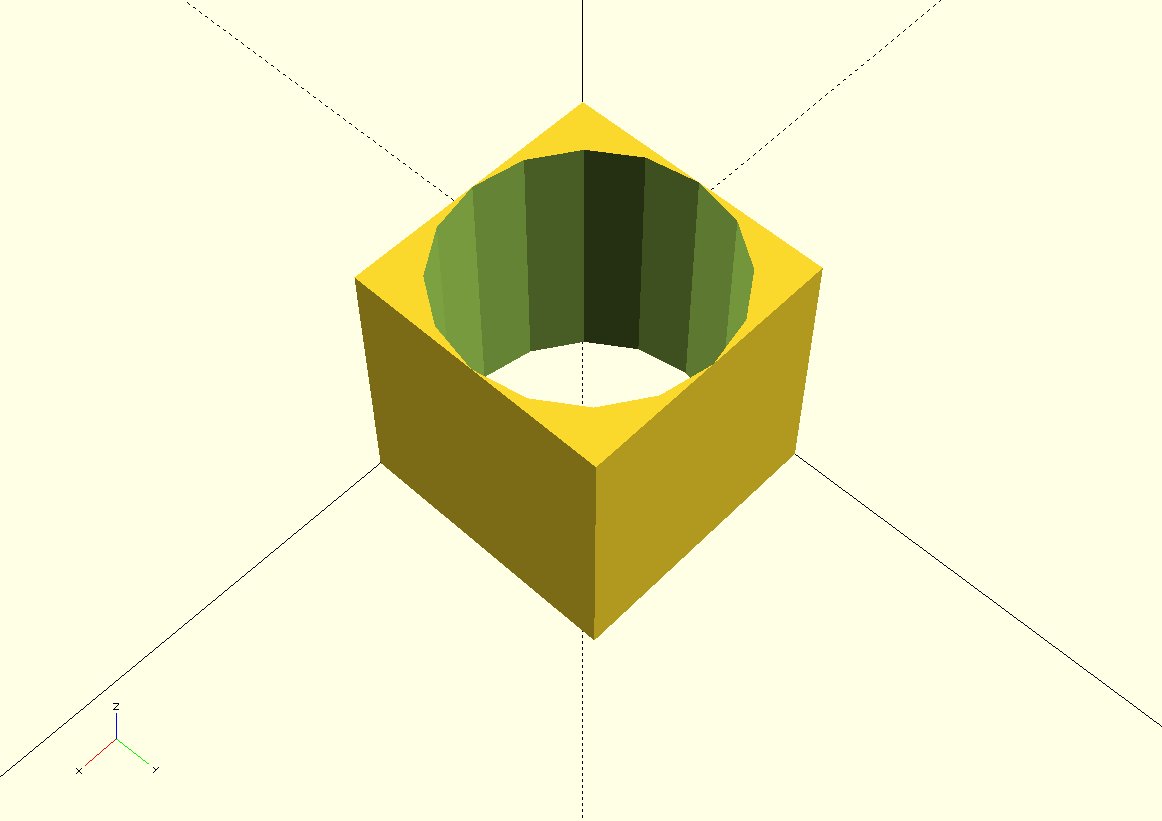
\includegraphics[width= 290px]{Bilder/OpenSCAD_Example}
\end{Bild}

Neben solchen einfachen Objekten wird außerdem die Möglichkeit geboten, komplexere Objekte wie Polygone (\icode{polygon()}) zu erstellen.
Diese können dann ausgehend von einem zweidimensionalen Polygon in Prismen umgewandelt werden (\icode{linear\_extrude()}). \\
Die Anweisungen, welche OpenSCAD zum Modellieren verwendet, werden in einfachen Textdateien im .scad-Format gespeichert.
Die Einfachheit dieser Textdateien erlaubt es, die erhaltenen Anweisungen ohne Umwandlungen in .scad-Dateien zu speichern, welche von OpenSCAD eingelesen, eingesehen und bearbeitet werden können. \\
%Drucken
Die Modelle, die mit OpenSCAD erstellt wurden, können anschließend mit einem 3D-Drucker ausgedruckt werden.
Dazu werden die Modelle in Dateien des .stl-Formats umgewandelt.
Die Konvertierung geschieht entweder über die Benutzeroberfläche von OpenSCAD oder mittels einer Kommandozeilenanweisung.

\section{3D-Drucker MakerBot Replicator\texttrademark\ 2}
%Erklärung 3D-Drucker
Der vorliegende 3D-Drucker ist vom Modell Replicator\texttrademark\ 2 der Firma MakerBot.
Dieser Drucker verfügt über eine höhenverstellbare Grundfläche, auf der das Filament\footnote{Filament bezeichnet das Material, welches der 3D-Drucker zum Drucken verwendet.} aufgetragen und das finale Objekt gedruckt wird.
Der Extruder erhitzt dazu das zu druckende Filament und trägt dieses auf die Grundfläche auf. 
Mithilfe dieser zwei Hauptbestandteile wird schichtweise Filament aufgetragen, welches aushärtet und so das Objekt bildet. \\
Die Höhe der Grundfläche wird während des Druckvorganges automatisch vom Drucker variiert und nach Abschluss des Drucks wieder auf den Ausgangszustand zurückgesetzt.
Um die Beweglichkeit des Extruders zu garantieren, ist dieser auf drei Achsen befestigt, sodass Motoren ihn auf diesen Achsen verschieben können. \\
Abhängig vom Filament bzw. der Temperatur, bei der dieses aufgetragen wird, der Bewegungsgeschwindigkeit des Extruders und der Filamentstärke, die der Extruder aufträgt, lässt sich die gewünschte Druckqualität anpassen.
Eine niedrige Qualität ist dabei mit einer kürzeren Druckzeit verbunden. \\
Die Druckzeit wird außerdem von der eingestellten Ausfüllung von geschlossenen Objekten und dem Hinzufügen von Druckhilfen beeinflusst.
So kann man Objekte beispielsweise nicht komplett mit Filament füllen lassen, sondern mit einem Bienenwabenmuster durchsetzen, sodass nur ein geringer Teil des Objektes ausgefüllt, aber dennoch Stabilität gewährleistet wird.
Indem so also ein stark verringerter Betrag an Filament aufgetragen werden muss, wird auch die Druckzeit drastisch reduziert. \\
Zu dem eigentlichen Druckergebnis wird unter jedes gedruckte Element eine dünne Schicht gedruckt, welcher leicht von der Grundplatte und vom gedruckten Modell zu trennen ist und so eine Beschädigung beim Entfernen des Objekts vom Drucker verhindert.
Außerdem werden bei Überhängen zusätzliche Stützen (\q{Supports}) gedruckt, um ein Absacken des noch nicht ausgehärteten Filaments zu verhindern.  \\
Beim Drucken von Objekten ist neben Anpassungen zur Kontrolle der Druckqualität und Druckzeit zu beachten, dass die Grundfläche begrenzt ist.
Entsprechend dieser vorgegebenen Maße sollten alle Objekte in ihrer Größe angepasst werden.
% [28.5 x 15.3 x 15.5 cm]